% ===========================================================================
%  TikuOS — TikuKits ML: Naive Bayes for Embedded Systems
%  Beamer Presentation
% ===========================================================================
\documentclass[aspectratio=169, 10pt]{beamer}

% ---- Theme ----------------------------------------------------------------
\usetheme{Madrid}
\usecolortheme{whale}
\setbeamertemplate{navigation symbols}{}
\setbeamertemplate{footline}{%
  \leavevmode\hbox{%
    \begin{beamercolorbox}[wd=.33\paperwidth,ht=2.5ex,dp=1ex,center]{author in head/foot}%
      \usebeamerfont{author in head/foot}\insertshortauthor
    \end{beamercolorbox}%
    \begin{beamercolorbox}[wd=.34\paperwidth,ht=2.5ex,dp=1ex,center]{title in head/foot}%
      \usebeamerfont{title in head/foot}\insertshorttitle
    \end{beamercolorbox}%
    \begin{beamercolorbox}[wd=.33\paperwidth,ht=2.5ex,dp=1ex,right]{date in head/foot}%
      \usebeamerfont{date in head/foot}\insertshortdate{}\hspace*{2em}%
      \insertframenumber{}/\inserttotalframenumber\hspace*{2ex}
    \end{beamercolorbox}}%
  \vskip0pt%
}

% ---- Packages -------------------------------------------------------------
\usepackage{listings}
\usepackage{graphicx}
\usepackage{hyperref}
\usepackage{booktabs}
\usepackage{multirow}
\usepackage{tikz}
\usetikzlibrary{arrows.meta, positioning, shapes.geometric, calc,
                decorations.pathreplacing, fit}
\usepackage{amsmath}

% ---- Code listing style ---------------------------------------------------
\lstset{
  basicstyle=\ttfamily\scriptsize,
  keywordstyle=\color{blue}\bfseries,
  commentstyle=\color{gray},
  stringstyle=\color{red!70!black},
  showstringspaces=false,
  breaklines=true,
  frame=single,
  rulecolor=\color{black!30},
  backgroundcolor=\color{blue!3},
  tabsize=4,
}
\lstdefinestyle{cstyle}{
  language=C,
  morekeywords={uint8_t,uint16_t,uint32_t,int32_t,int64_t,
                tiku_kits_ml_elem_t,
                TIKU_KITS_ML_OK,TIKU_KITS_ML_ERR_NULL,
                TIKU_KITS_ML_ERR_SIZE,TIKU_KITS_ML_ERR_PARAM,
                TIKU_KITS_ML_NBAYES_MAX_CLASSES,
                TIKU_KITS_ML_NBAYES_MAX_FEATURES,
                TIKU_KITS_ML_NBAYES_MAX_BINS,
                TIKU_KITS_ML_NBAYES_SHIFT,
                NULL},
}

% ---- Metadata -------------------------------------------------------------
\title[TikuKits ML]{TikuKits ML: Naive Bayes for Embedded Systems}
\subtitle{Simple. Ubiquitous. Intelligence, Everywhere.}
\author[Ambuj Varshney]{Ambuj Varshney \\ \texttt{ambuj@tiku-os.org}}
\date{\today}

% ===========================================================================
\begin{document}

% ---------------------------------------------------------------------------
\begin{frame}
\titlepage
\end{frame}

% ---------------------------------------------------------------------------
\begin{frame}{Outline}
\tableofcontents
\end{frame}

% ===========================================================================
\section{Motivation}
% ===========================================================================

\begin{frame}{Why Naive Bayes on MCUs?}
\begin{columns}[T]
\begin{column}{0.48\textwidth}
\begin{block}{Embedded Use Cases}
\begin{itemize}
  \item \textbf{Categorical sensor data} --- binned ADC readings
  \item \textbf{Activity recognition} --- motion state classification
  \item \textbf{Fast training} --- single-pass frequency counting
  \item \textbf{Multi-class} --- handles 2+ classes naturally
\end{itemize}
\end{block}

\begin{block}{Constraints}
\begin{itemize}
  \item No FPU (16-bit MSP430)
  \item No heap allocation
  \item Limited RAM (2--8\,KB)
  \item No \texttt{exp()}, \texttt{log()}, or \texttt{sqrt()}
\end{itemize}
\end{block}
\end{column}

\begin{column}{0.48\textwidth}
\begin{center}
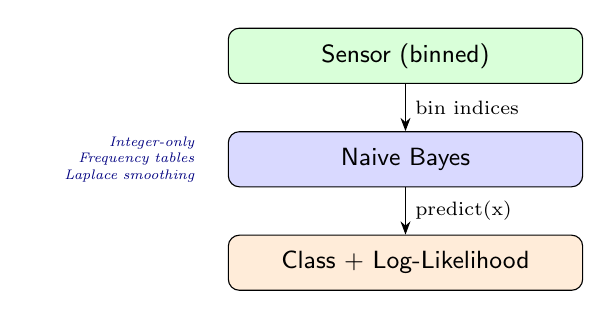
\begin{tikzpicture}[
    >=Stealth, node distance=0.5cm
  ]
  \node[draw, rounded corners, minimum height=0.7cm,
        text centered, font=\small\sffamily, fill=green!15,
        minimum width=4.5cm] (sensor) {Sensor (binned)};
  \node[draw, rounded corners, minimum height=0.7cm,
        text centered, font=\small\sffamily, fill=blue!15,
        minimum width=4.5cm, below=0.6cm of sensor] (nb)
    {Naive Bayes};
  \node[draw, rounded corners, minimum height=0.7cm,
        text centered, font=\small\sffamily, fill=orange!15,
        minimum width=4.5cm, below=0.6cm of nb] (output)
    {Class + Log-Likelihood};
  \draw[->] (sensor) -- node[right, font=\scriptsize] {bin indices} (nb);
  \draw[->] (nb) -- node[right, font=\scriptsize] {predict(x)} (output);

  \node[left=0.3cm of nb, font=\tiny\itshape, text=blue!50!black,
        text width=2cm, align=right] {Integer-only\\Frequency tables\\Laplace smoothing};
\end{tikzpicture}
\end{center}

\vspace{0.5em}
\begin{alertblock}{Design Goal}
Categorical Naive Bayes using \textbf{frequency tables} and
\textbf{integer log$_2$} approximation. No floating point,
no transcendental functions.
\end{alertblock}
\end{column}
\end{columns}
\end{frame}

% ===========================================================================
\section{Algorithm Theory}
% ===========================================================================

\begin{frame}{Categorical Naive Bayes}
\begin{columns}[T]
\begin{column}{0.48\textwidth}
\textbf{Bayes' theorem:}
\[
  P(c \mid \mathbf{x}) \propto P(c) \prod_{j=1}^{n} P(x_j \mid c)
\]

\textbf{Log-space scoring} (avoids products of small numbers):
\[
  \text{score}(c) = \log_2 P(c) + \sum_{j=1}^{n} \log_2 P(x_j \mid c)
\]

\textbf{With Laplace smoothing:}
\[
  P(x_j = v \mid c) = \frac{\text{freq}[c][j][v] + 1}{\text{count}_c + B}
\]
where $B$ = number of bins.

\vspace{0.3em}
\textbf{Prediction:} $\hat{y} = \arg\max_c \text{score}(c)$
\end{column}

\begin{column}{0.48\textwidth}
\begin{block}{Integer $\log_2$ Approximation}
Uses a bit-scan (count leading zeros) to compute
$\lfloor \log_2(n) \rfloor$ in Q(shift):
\[
  \text{log2\_q}(n) = \lfloor \log_2(n) \rfloor \times 2^{\text{shift}}
\]
No floating point, no lookup tables larger than a word.
\end{block}

\vspace{0.3em}
\begin{block}{Frequency Table}
\begin{center}
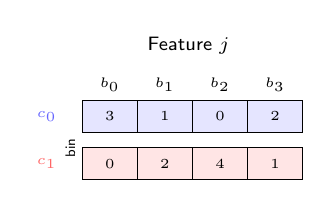
\begin{tikzpicture}[
    cell/.style={draw, minimum width=0.7cm, minimum height=0.4cm,
                 font=\tiny}
  ]
  \node[font=\tiny\sffamily, rotate=90] at (-0.5, 0.2) {bin};
  \node[cell, fill=blue!10] at (0, 0.6) {3};
  \node[cell, fill=blue!10] at (0.7, 0.6) {1};
  \node[cell, fill=blue!10] at (1.4, 0.6) {0};
  \node[cell, fill=blue!10] at (2.1, 0.6) {2};

  \node[cell, fill=red!10] at (0, 0) {0};
  \node[cell, fill=red!10] at (0.7, 0) {2};
  \node[cell, fill=red!10] at (1.4, 0) {4};
  \node[cell, fill=red!10] at (2.1, 0) {1};

  \node[font=\tiny] at (0, 1.0) {$b_0$};
  \node[font=\tiny] at (0.7, 1.0) {$b_1$};
  \node[font=\tiny] at (1.4, 1.0) {$b_2$};
  \node[font=\tiny] at (2.1, 1.0) {$b_3$};

  \node[font=\tiny, blue!60] at (-0.8, 0.6) {$c_0$};
  \node[font=\tiny, red!60] at (-0.8, 0) {$c_1$};

  \node[font=\scriptsize\sffamily] at (1.0, 1.5) {Feature $j$};
\end{tikzpicture}
\end{center}
One table per (class, feature) pair.
\end{block}
\end{column}
\end{columns}
\end{frame}

% ===========================================================================
\section{Data Structure}
% ===========================================================================

\begin{frame}[fragile]{The \texttt{tiku\_kits\_ml\_nbayes} Structure}
\begin{columns}[T]
\begin{column}{0.48\textwidth}
\begin{lstlisting}[style=cstyle,
  title={ml/classification/tiku\_kits\_ml\_nbayes.h}]
struct tiku_kits_ml_nbayes {
    uint16_t freq
        [TIKU_KITS_ML_NBAYES_MAX_CLASSES]
        [TIKU_KITS_ML_NBAYES_MAX_FEATURES]
        [TIKU_KITS_ML_NBAYES_MAX_BINS];
    uint16_t class_count
        [TIKU_KITS_ML_NBAYES_MAX_CLASSES];
    uint16_t n_total;
    uint8_t  n_features;
    uint8_t  n_bins;
    uint8_t  n_classes;
    uint8_t  shift;
};
\end{lstlisting}

\textbf{Memory footprint:}\\
$4 \times 4 \times 16 \times 2 + 4 \times 2 + 2 + 4$\\
$= 522$ bytes (default config).
\end{column}

\begin{column}{0.48\textwidth}
\begin{lstlisting}[style=cstyle,
  title={Configuration macros}]
/* Max output classes */
#ifndef TIKU_KITS_ML_NBAYES_MAX_CLASSES
#define TIKU_KITS_ML_NBAYES_MAX_CLASSES 4
#endif

/* Max input features */
#ifndef TIKU_KITS_ML_NBAYES_MAX_FEATURES
#define TIKU_KITS_ML_NBAYES_MAX_FEATURES 4
#endif

/* Max bins per feature */
#ifndef TIKU_KITS_ML_NBAYES_MAX_BINS
#define TIKU_KITS_ML_NBAYES_MAX_BINS 16
#endif

/* Default Q-format shift */
#ifndef TIKU_KITS_ML_NBAYES_SHIFT
#define TIKU_KITS_ML_NBAYES_SHIFT 8
#endif
\end{lstlisting}
\end{column}
\end{columns}
\end{frame}

% ===========================================================================
\section{API Reference}
% ===========================================================================

\begin{frame}[fragile]{Complete API}
\begin{table}
\centering
\small
\begin{tabular}{@{}lp{8cm}@{}}
\toprule
\textbf{Function} & \textbf{Description} \\
\midrule
\texttt{tiku\_kits\_ml\_nbayes\_init(nb, nf, nb, nc, sh)}
  & Initialize with \texttt{nf} features, \texttt{nb} bins,
    \texttt{nc} classes, Q-format \texttt{sh} \\
\texttt{tiku\_kits\_ml\_nbayes\_reset(nb)}
  & Clear all frequency tables and counts \\
\midrule
\texttt{tiku\_kits\_ml\_nbayes\_train(nb, x, y)}
  & Train: increment frequency counts for binned features \\
\texttt{tiku\_kits\_ml\_nbayes\_predict(nb, x, \&result)}
  & Return class with highest log-likelihood \\
\texttt{tiku\_kits\_ml\_nbayes\_predict\_log\_proba(nb, x, s)}
  & Return all class log-likelihood scores in Q(shift) \\
\midrule
\texttt{tiku\_kits\_ml\_nbayes\_count(nb)}
  & Total number of training samples seen \\
\bottomrule
\end{tabular}
\end{table}

\vspace{0.3em}
\begin{alertblock}{Input Format}
Features must be \textbf{pre-binned} to \texttt{uint8\_t} values in
$[0, \text{n\_bins})$. The caller is responsible for discretizing
continuous sensor values into bin indices before calling
\texttt{train()} or \texttt{predict()}.
\end{alertblock}
\end{frame}

% ===========================================================================
\section{Implementation Details}
% ===========================================================================

\begin{frame}[fragile]{Training and Prediction}
\begin{columns}[T]
\begin{column}{0.48\textwidth}
\begin{lstlisting}[style=cstyle,
  title={Training: frequency counting}]
int tiku_kits_ml_nbayes_train(
    struct tiku_kits_ml_nbayes *nb,
    const uint8_t *x,
    uint8_t y)
{
    uint8_t j;

    /* Increment per-feature bin count */
    for (j = 0; j < nb->n_features; j++) {
        nb->freq[y][j][x[j]]++;
    }

    /* Increment class and total counts */
    nb->class_count[y]++;
    nb->n_total++;

    return TIKU_KITS_ML_OK;
}
\end{lstlisting}

\vspace{0.3em}
\textbf{O(n\_features)} per training sample.\\
No matrix operations, no gradient descent.
\end{column}

\begin{column}{0.48\textwidth}
\begin{lstlisting}[style=cstyle,
  title={Prediction: log-likelihood scoring}]
/* For each class c: */
score = log2_q(class_count[c]);

for (j = 0; j < n_features; j++) {
    /* Laplace-smoothed likelihood */
    score += log2_q(
        freq[c][j][x[j]] + 1);
    score -= log2_q(
        class_count[c] + n_bins);
}

/* Predict: argmax over all scores */
\end{lstlisting}

\vspace{0.3em}
\begin{block}{Laplace Smoothing}
Adding 1 to numerator and $B$ to denominator
prevents zero-probability bins from dominating.
Critical for sparse data on embedded targets.
\end{block}
\end{column}
\end{columns}
\end{frame}

% ===========================================================================
\section{Examples}
% ===========================================================================

\begin{frame}[fragile]{Example 1: Temperature Zone Classification}
\begin{lstlisting}[style=cstyle,
  title={examples/example\_ml\_nbayes.c --- 3 zones, 5 bins}]
struct tiku_kits_ml_nbayes nb;
uint8_t result;

/* 1 feature, 5 bins, 3 classes, Q8 */
tiku_kits_ml_nbayes_init(&nb, 1, 5, 3, 8);

/* Bin mapping: [0..100)->0, [100..200)->1, [200..300)->2,
 *              [300..400)->3, [400+)->4 */

/* Train: cold=0, normal=1, hot=2 */
uint8_t cold_bins[]   = {0, 0, 1, 0, 1};    /* low bins */
uint8_t normal_bins[] = {2, 2, 2, 1, 2};    /* mid bins */
uint8_t hot_bins[]    = {3, 4, 3, 4, 3};    /* high bins */

uint8_t i;
for (i = 0; i < 5; i++) {
    tiku_kits_ml_nbayes_train(&nb, &cold_bins[i],   0);
    tiku_kits_ml_nbayes_train(&nb, &normal_bins[i], 1);
    tiku_kits_ml_nbayes_train(&nb, &hot_bins[i],    2);
}

/* Classify: bin 2 -> normal */
uint8_t query = 2;
tiku_kits_ml_nbayes_predict(&nb, &query, &result);  /* result = 1 */
\end{lstlisting}
\end{frame}

% ---------------------------------------------------------------------------
\begin{frame}[fragile]{Example 2: Activity Recognition}
\begin{columns}[T]
\begin{column}{0.52\textwidth}
\begin{lstlisting}[style=cstyle,
  title={2-feature: magnitude + frequency}]
struct tiku_kits_ml_nbayes nb;
uint8_t result;
int32_t scores[3];

/* 2 features, 4 bins, 3 classes, Q8 */
tiku_kits_ml_nbayes_init(&nb, 2, 4, 3, 8);

/* sitting=0: low mag, low freq */
uint8_t sit1[] = {0, 0};
uint8_t sit2[] = {0, 1};
tiku_kits_ml_nbayes_train(&nb, sit1, 0);
tiku_kits_ml_nbayes_train(&nb, sit2, 0);

/* walking=1: med mag, med freq */
uint8_t walk1[] = {1, 2};
uint8_t walk2[] = {2, 2};
tiku_kits_ml_nbayes_train(&nb, walk1, 1);
tiku_kits_ml_nbayes_train(&nb, walk2, 1);

/* running=2: high mag, high freq */
uint8_t run1[] = {3, 3};
uint8_t run2[] = {3, 2};
tiku_kits_ml_nbayes_train(&nb, run1, 2);
tiku_kits_ml_nbayes_train(&nb, run2, 2);

/* Classify */
uint8_t q[] = {1, 1};
tiku_kits_ml_nbayes_predict(&nb, q, &result);

/* Inspect scores */
tiku_kits_ml_nbayes_predict_log_proba(
    &nb, q, scores);
\end{lstlisting}
\end{column}

\begin{column}{0.44\textwidth}
\begin{center}
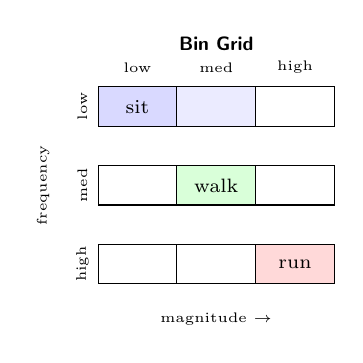
\begin{tikzpicture}[
    cell/.style={draw, minimum width=1.0cm, minimum height=0.5cm,
                 font=\scriptsize, text centered}
  ]
  \node[font=\scriptsize\sffamily\bfseries] at (1.5, 2.3) {Bin Grid};

  \node[cell, fill=blue!15] at (0.5, 1.5) {sit};
  \node[cell, fill=blue!8] at (1.5, 1.5) {};
  \node[cell, fill=white] at (2.5, 1.5) {};
  \node[cell, fill=white] at (0.5, 0.5) {};
  \node[cell, fill=green!15] at (1.5, 0.5) {walk};
  \node[cell, fill=white] at (2.5, 0.5) {};
  \node[cell, fill=white] at (0.5, -0.5) {};
  \node[cell, fill=white] at (1.5, -0.5) {};
  \node[cell, fill=red!15] at (2.5, -0.5) {run};

  \node[font=\tiny] at (0.5, 2.0) {low};
  \node[font=\tiny] at (1.5, 2.0) {med};
  \node[font=\tiny] at (2.5, 2.0) {high};

  \node[font=\tiny, rotate=90] at (-0.2, 1.5) {low};
  \node[font=\tiny, rotate=90] at (-0.2, 0.5) {med};
  \node[font=\tiny, rotate=90] at (-0.2, -0.5) {high};

  \node[font=\tiny] at (1.5, -1.2) {magnitude $\rightarrow$};
  \node[font=\tiny, rotate=90] at (-0.7, 0.5) {frequency};
\end{tikzpicture}
\end{center}

\vspace{0.5em}
\begin{block}{Log-Likelihood Scores}
\texttt{predict\_log\_proba()} returns
per-class scores in Q(shift).
Higher score = more likely class.
Useful for confidence thresholding.
\end{block}
\end{column}
\end{columns}
\end{frame}

% ===========================================================================
\section{Test Suite}
% ===========================================================================

\begin{frame}{Test Cases Overview}
\begin{table}
\centering
\small
\begin{tabular}{@{}clp{7cm}@{}}
\toprule
\textbf{\#} & \textbf{Test Function} & \textbf{What It Verifies} \\
\midrule
1 & \texttt{test\_kits\_ml\_nbayes\_init}
  & Initialization, parameter bounds validation \\
2 & \texttt{test\_kits\_ml\_nbayes\_simple}
  & 1-feature, 2-class classification \\
3 & \texttt{test\_kits\_ml\_nbayes\_two\_features}
  & 2-feature classification \\
4 & \texttt{test\_kits\_ml\_nbayes\_three\_class}
  & 3-class classification \\
5 & \texttt{test\_kits\_ml\_nbayes\_log\_proba}
  & Log-likelihood score output \\
6 & \texttt{test\_kits\_ml\_nbayes\_smoothing}
  & Laplace smoothing on unseen bins \\
7 & \texttt{test\_kits\_ml\_nbayes\_imbalanced}
  & Class imbalance handling (prior effect) \\
8 & \texttt{test\_kits\_ml\_nbayes\_reset}
  & Reset clears all frequency tables \\
9 & \texttt{test\_kits\_ml\_nbayes\_null\_inputs}
  & All functions reject NULL with ERR\_NULL \\
\bottomrule
\end{tabular}
\end{table}
\end{frame}

% ===========================================================================
\section{Summary}
% ===========================================================================

\begin{frame}{Summary}
\begin{columns}[T]
\begin{column}{0.48\textwidth}
\begin{block}{What We Built}
\begin{itemize}
  \item Categorical Naive Bayes classifier
  \item Frequency-table based (no matrix ops)
  \item Integer $\log_2$ scoring (no FPU)
  \item Laplace smoothing for robustness
  \item $\sim$522 bytes state (default config)
\end{itemize}
\end{block}

\begin{block}{Key Design Choices}
\begin{itemize}
  \item Pre-binned input (caller discretizes)
  \item Log-space scoring avoids tiny products
  \item Bit-scan $\log_2$ replaces \texttt{log()}
  \item Smoothing prevents zero-probability bins
\end{itemize}
\end{block}
\end{column}

\begin{column}{0.48\textwidth}
\begin{block}{Use Cases}
\begin{itemize}
  \item Temperature zone classification
  \item Activity recognition (sit/walk/run)
  \item Categorical sensor pattern matching
  \item Multi-class embedded decisions
\end{itemize}
\end{block}

\begin{block}{Files}
\scriptsize
\begin{tabular}{@{}lp{4.5cm}@{}}
Header: & \texttt{ml/classification/tiku\_kits\_ml\_nbayes.h} \\
Source: & \texttt{ml/classification/tiku\_kits\_ml\_nbayes.c} \\
Tests: & \texttt{tests/ml/test\_kits\_ml\_nbayes.c} \\
Example: & \texttt{examples/example\_ml\_nbayes.c} \\
\end{tabular}
\end{block}
\end{column}
\end{columns}
\end{frame}

% ---------------------------------------------------------------------------
\begin{frame}{Thank You}
\begin{center}
\Large\textbf{TikuKits ML: Naive Bayes}\\[0.5em]
\normalsize Integer-Only Machine Learning for Physical AI Endpoints\\[1.5em]

\begin{tabular}{rl}
  Repository: & \url{https://github.com/tikuos/tikuOS} \\
  License:    & Apache 2.0 \\
  Common:     & \texttt{tikukits/ml/tiku\_kits\_ml.h} \\
  Header:     & \texttt{tikukits/ml/classification/tiku\_kits\_ml\_nbayes.h} \\
  Source:     & \texttt{tikukits/ml/classification/tiku\_kits\_ml\_nbayes.c} \\
  Tests:      & \texttt{tikukits/tests/ml/test\_kits\_ml\_nbayes.c} \\
  Examples:   & \texttt{tikukits/examples/example\_ml\_nbayes.c} \\
\end{tabular}
\end{center}
\end{frame}

\end{document}
